\documentclass[a4paper, 12pt]{article}
\usepackage[a4paper,top=1.5cm, bottom=1.5cm, left=1cm, right=1cm]{geometry}
\usepackage{cmap}					
\usepackage{mathtext} 				
\usepackage[T2A]{fontenc}			
\usepackage[utf8]{inputenc}			
\usepackage[english,russian]{babel}
\usepackage{multirow}
\usepackage{graphicx}
\usepackage{wrapfig}
\usepackage{tabularx}
\usepackage{float}
\usepackage{longtable}
\usepackage{hyperref}
\hypersetup{colorlinks=true,urlcolor=blue}
\usepackage[rgb]{xcolor}
\usepackage{amsmath,amsfonts,amssymb,amsthm,mathtools} 
\usepackage{icomma} 
\usepackage{euscript}
\usepackage{mathrsfs}
\usepackage{enumerate}
\usepackage{caption}
\usepackage{enumerate}
\mathtoolsset{showonlyrefs=true}
\usepackage{graphicx}
\usepackage{caption}
\usepackage{subcaption}
\usepackage[europeanresistors, americaninductors]{circuitikz}
\DeclareMathOperator{\sgn}{\mathop{sgn}}
\newcommand*{\hm}[1]{#1\nobreak\discretionary{}
	{\hbox{$\mathsurround=0pt #1$}}{}}

\begin{document}

\newgeometry{left=2cm, right=2cm, top=2cm, bottom=1cm, bindingoffset=0cm}
\begin{titlepage}
    
    \begin{center}

        \vspace*{5cm}
        \Huge МФТИ
        \vspace*{2cm}\\
        \LARGE Вопрос по выбору
        \\\vspace*{0.25cm}
        
        \noindent\rule{\textwidth}{1pt}
        \vspace*{-0.25cm}
        
        \huge \textbf{Изучение падения пружины слинки (slinky)}
        \noindent\rule{\textwidth}{1pt}


       \vfill

        \begin{flushright}
            \begin{minipage}{.4\textwidth}
            \Large Выполнили: \\ Манро Эйден      \\ (Б01-308) 
                              \\ Солодилов Михаил \\ (Б01-307)
            \end{minipage}
        \end{flushright}
        
        \vfill

        \normalsize Долгопрудный \\2024
        
    \end{center}

\end{titlepage}
\restoregeometry

\begin{center}
    \section*{Введение}
\end{center}


\noindent \textbf{Цель работы:} исследовать некоторые динамические параметры слинки: время шага, отношение массы пружинки, участвующей в движении к её полной массе; проверить схожесть теоретических и экспериментальных результатов.  

\bigskip

\noindent \textbf{Оборудование:} слинки, лестница, сооруженная из коробок, cекундомер, линейка.
\bigskip


% \begin{center}
% \subsection*{История}
% \end{center}

$\>$ Слинки — игрушка-пружина, созданная в 1943 году в США Ричардом Джеймсом. 
Это пружинка с очень малым коэффициентом упругости, диаметр ее витков — от 5 до 10 см, количество витков — от 30 до 100.
А именно это свойство и позволяет проводить с ней интересные опыты, которые невозможны с обычной пружинкой. Самое любопытное заключается в том, что слинки может спускаться по ступенькам лестницы (или по наклонной плоскости). Достаточно, установив слинки в вертикальном положении на краю ступеньки, подтолкнуть ее верхний конец в направлении нижней ступеньки, и слинки зашагает. Пружинка будет как бы перетекать с верхней ступеньки на нижнюю. Когда вся пружинка перетечет, верхний конец, описав в воздухе дугу, шагнет на следующую ступеньку, и движение продолжится. 

% \begin{center}
% \section*{Ход работы}
% \end{center}

% \begin{center}    
% \subsection*{Исходные данные}
% \end{center}

\begin{table}[h]
    \begin{center}
    \begin{tabular}{|c|c|c|c|}
        \hline \hline
        $ N $ & $ M, \text{г} $ & $ l_{0}, \text{см} $ & $ L_{0}, \text{см}$ \\
        \hline
        38 & 35 & 6.1 & 120.0 \\
        \hline \hline
    \end{tabular}
    \caption{Данные системы}
    \end{center}
\end{table}

\begin{itemize}
    \item $ N $ - количество витков. 
    \item $ M $ - масса пружины. 
    \item $ l_{0} $ - высота пружины в недеформированном состоянии.
    \item $ L_{0} $ - длина пружины растянутой под собственным весом.
\end{itemize}

\begin{center}    
\subsection*{Погрешности}
\end{center}

\begin{itemize}
	\item \textbf{Линейка:} $ \sigma_\text{лин} = 0.5 $ мм
	\item \textbf{Видеокамера:} $ \sigma_\text{сек} = 0.008 $ с
	\item \textbf{Электронные весы:} $ \sigma_\text{вес} = 1 $ г
\end{itemize}

$\>$ Подвесим свободно слинки за верхний конец и найдем зависимость линейной плотности пружинки, что пропорционально числу витков на единицу длины,
от расстояния до нижнего конца. 

\bigskip

$\>$ Рассмотрим некоторый участок пружинки. Пусть он находится на n-й виток,
считая от нижнего конца пружинки. Если длина этого витка равна $\varDelta x_{n}$, то:

\begin{equation}
    \varDelta k \varDelta x_{n} = \varDelta m n g,    
\end{equation}

\bigskip

где $\varDelta k$ жесткость одного витка, $\varDelta m $ его масса соответственно.

\bigskip

Тогда получаем, что средняя линейная плотность n-го витка равна:

\bigskip

\begin{equation}
    \lambda_{n} = \frac{\varDelta m}{\varDelta x_{n}} = \frac{\varDelta k}{ng}
\end{equation}

\bigskip

Теперь найдем расстояние от этого витка до нижнего конца пружины:

\bigskip

\begin{equation}
    x_{n} = \sum_{i=1}^{n} \frac{\varDelta m g}{\varDelta k} i = \frac{\varDelta mg}{\varDelta k} \frac{n(n+1)}{2} 
\end{equation}

\bigskip

Так как жесткость последовательно соединённых пружин равна обратной сумме обратных жетскостей, т.е.:

\bigskip

\begin{equation}
    \frac{1}{k} = \sum_{i = 1}^{n} \frac{1}{\varDelta k_{i}} \; \rightarrow \; \varDelta k \cdot n = k
\end{equation}

Получаем, что:

\bigskip

\begin{equation}
    x_{n} = \frac{Mg}{2k} \frac{n(n+1)}{N^2} \approx \frac{Mg}{2k} \frac{n^2}{N^2},
\end{equation}

\bigskip

Если мы подставим в качестве $ n = N $, то получим формулу для длины $ L_{0} $ пружины:

\bigskip

\begin{equation}  
    L_{0} = \frac{Mg}{2k} \label{length} 
\end{equation}  

\bigskip

Отсюда найдём жесткость пружины:

\bigskip

\begin{equation}
    k = \frac{Mg}{2L_{0}}, \; \;
    \sigma_{k} = k \sqrt{\bigg(\frac{\sigma_{M}}{M}\bigg)^2 + \bigg(\frac{\sigma_{L_{0}}}{L_{0}}\bigg)^2}
\end{equation}

\bigskip

\begin{center}
    \textbf{Итого:} \underline{$ k = 0.1430 \pm 0.0037 \; [\frac{\text{Н}}{\text{кг}}] $} $ \; (\varepsilon = 2.6 \%) $  
\end{center}

\bigskip

Найдём зависимость для линейной плотности $ \lambda_{n} $ и расстояния $ x_{n} $:

\bigskip

\begin{equation}
    \lambda_{n} = \frac{kN}{gn} = \sqrt{\frac{Mk}{2gx_{n}}}
\end{equation}

\bigskip

Перейдя от дискретной записи распределения линейной плотности к непрерывной получаем:

\bigskip

\begin{equation}
    \lambda(x) = \sqrt{\frac{Mk}{2gx}}
\end{equation}

\bigskip

\begin{figure}[H]
    \begin{center}
        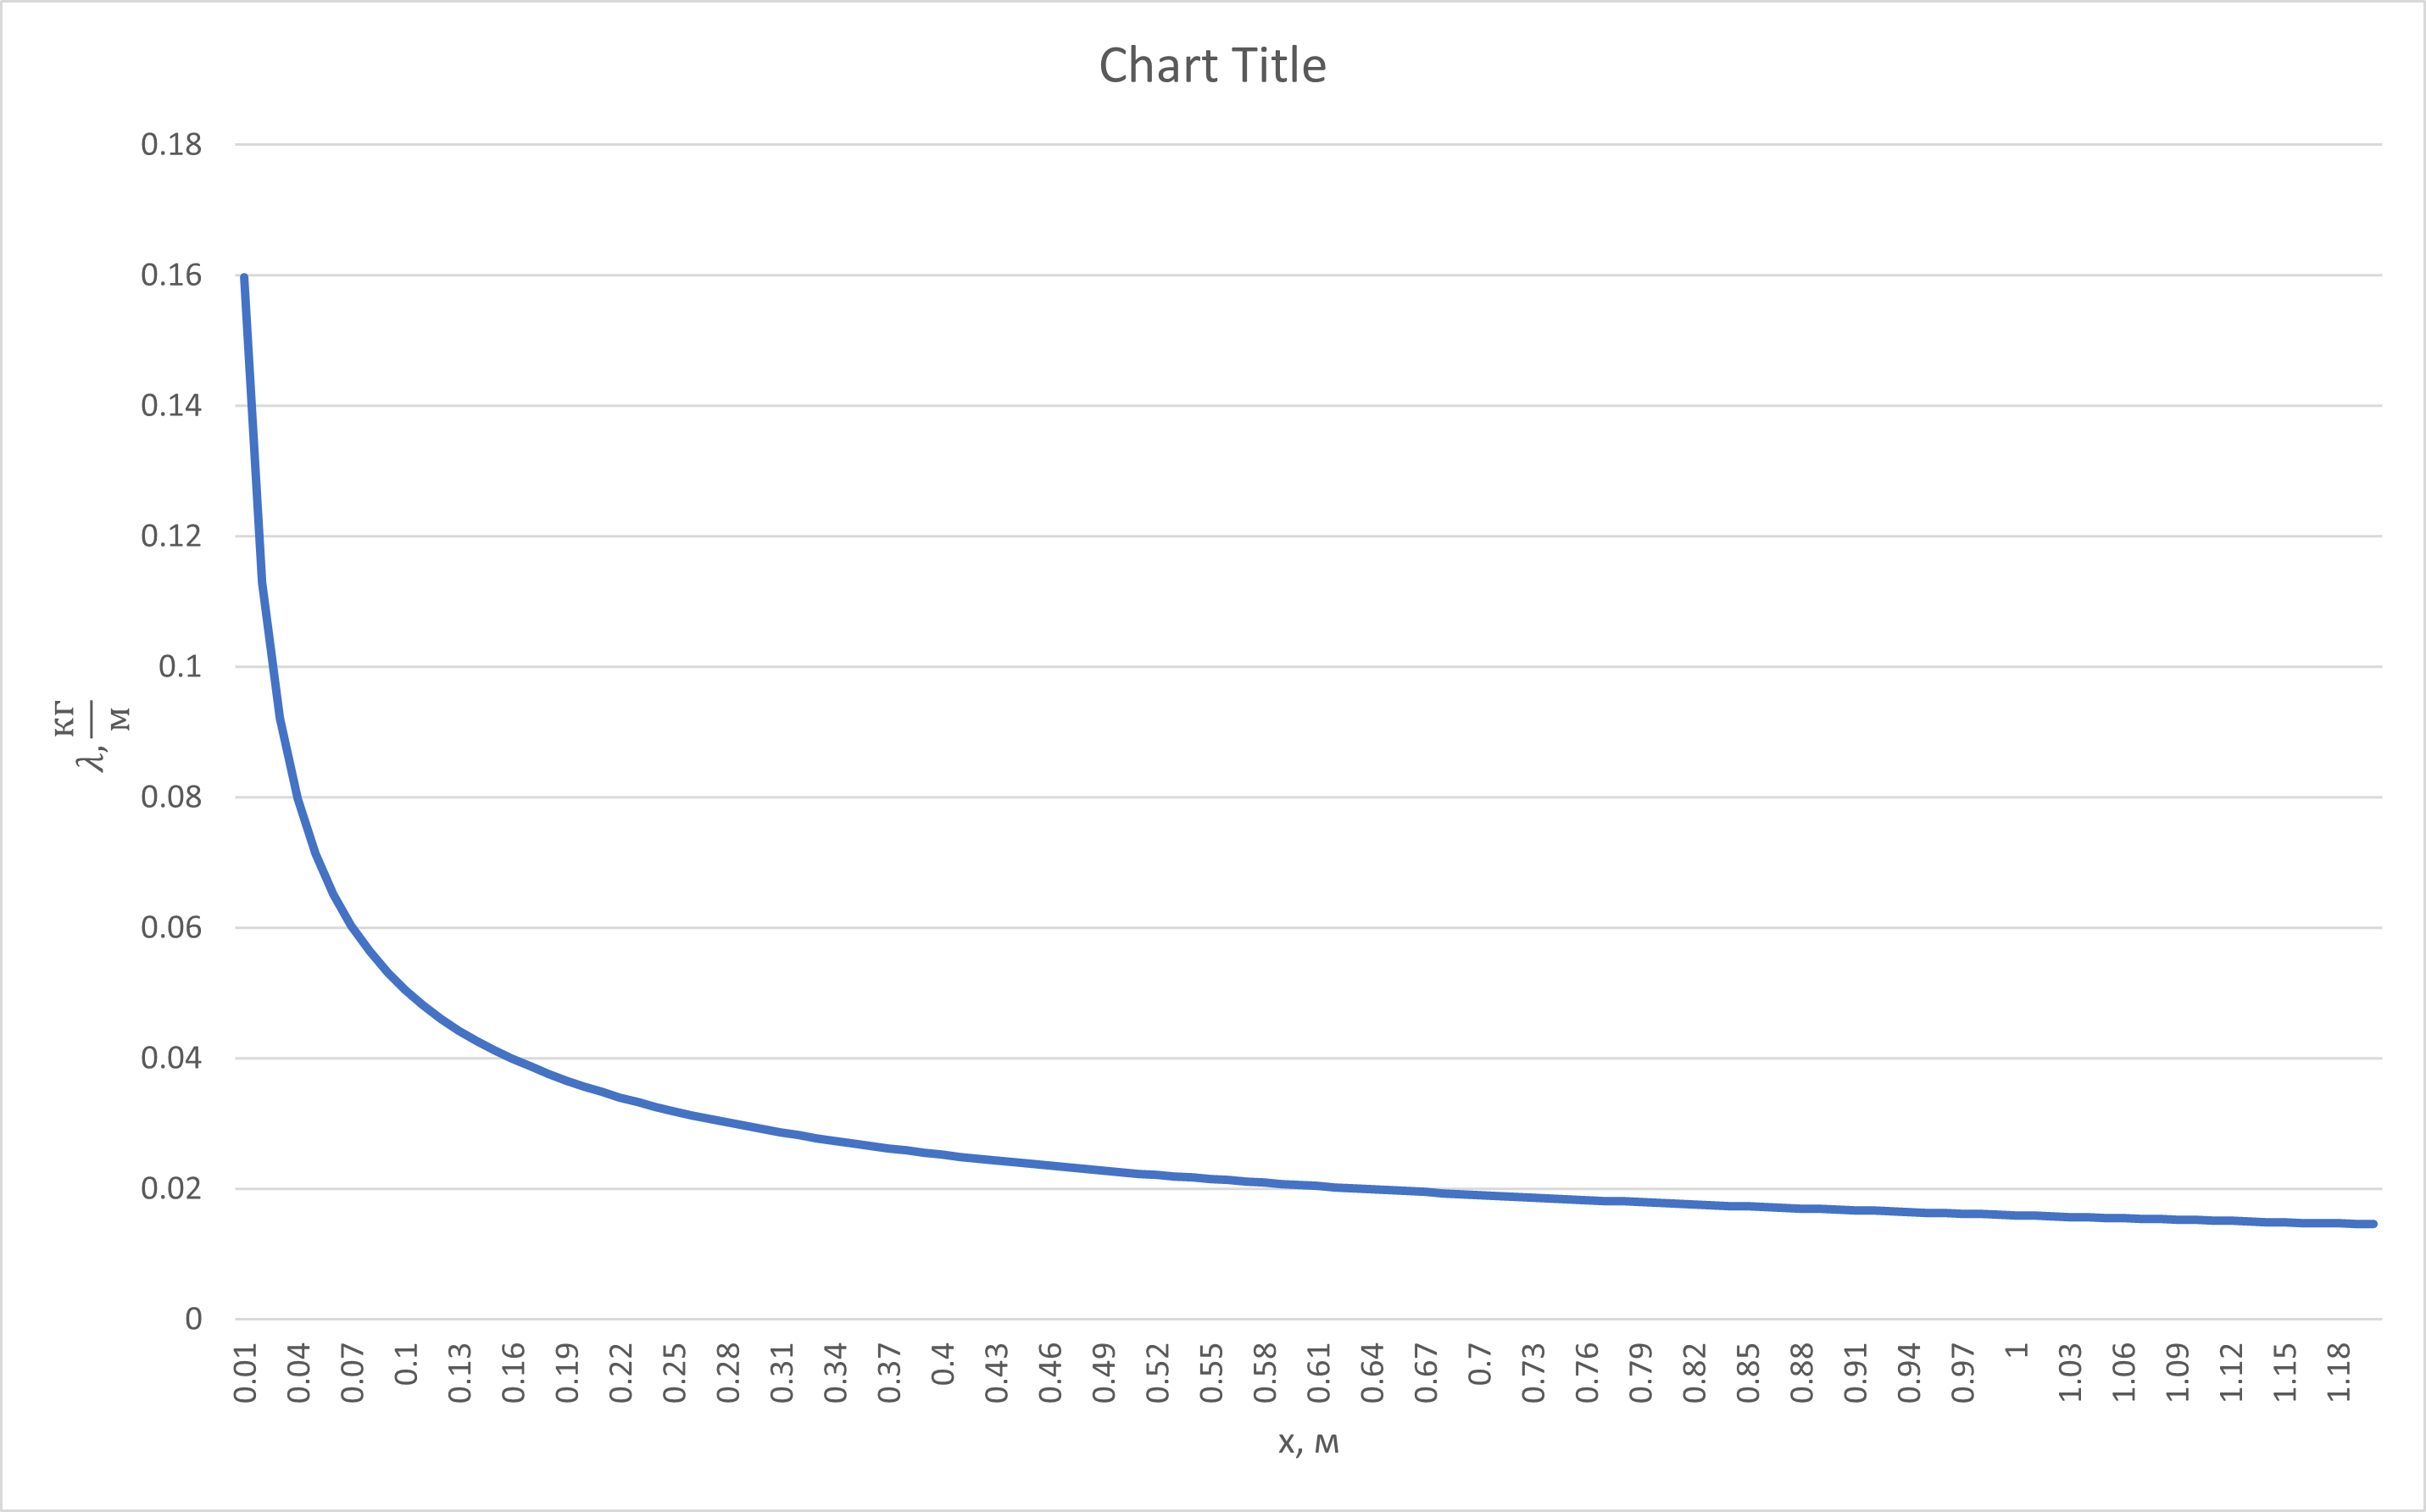
\includegraphics[width = 0.8\textwidth]{chart.png}
        \caption{График зависимости $\lambda(x)$}
    \end{center}
\end{figure}

\bigskip

Теперь мы можем оценить массу пружины, участвующей в движении. Будем считать, что искомая часть пружины эквивалентна свободно подвешенной пружине, длина которой - высота ступеньки $ h $. Используя только что полученную зависимость, оценим массу:

\bigskip

\begin{equation}
    m = \int_{0}^{h} \lambda(x) dx = \int_{0}^{h} \sqrt{\frac{Mk}{2gx}} dx = \sqrt{\frac{2Mkh}{g}}     
\end{equation}

\bigskip

Таким образом отношение массы, участвующей в движении, к полной:

\bigskip

\begin{equation}
    \frac{m}{M} = \sqrt{\frac{2kh}{Mg}} = \sqrt{\frac{h}{L_{0}}}
\end{equation}

Чтобы определить время одного шага слинки, воспользуемся вторым
законом Ньютона. Пусть начальная скорость верхнего витка $v$. Тогда

\[v\Delta{m} = F\Delta{t},\]

где $F$ — сила натяжения пружинки в верхней точке, $\Delta{m}$ —
масса пружинки, которая пришла в движение за время $\Delta{t}$.
Если $\lambda_0$ — линейная плотность пружинки в месте начала
движения, то  $\Delta{m} = \lambda_0v\Delta{t}$, и

\[\lambda_0v^2 = F\]

Поймём, что:

\[\lambda_0 = \sqrt{\frac{Mk}{2gh}}, \textup{а } F = m_0g = 
\sqrt{2Mgkh}\]

Поэтому для скорости «разматывания» получаем

\[v = \sqrt{\frac{F}{\lambda_0}} = \sqrt{2gh}.\]

Пусть за время $\Delta{t}$ «размоталась» часть пружинки массой
$\Delta{m} = \lambda_0v\Delta{t}$. Подставив значения
$\lambda_0$ и $v$, имеем:

\[\Delta{t} = \frac{\Delta{m}}{\sqrt{Mk}}.\]

Откуда получаем время одного шага слинки:

\[T = \sum{\Delta{t_i}} = \frac{1}{\sqrt{Mk}}\sum{\Delta{m_i}} =
\sqrt{\frac{M}{k}} = \sqrt{\frac{2L_0}{g}}.\]

\begin{center}
    \section*{Эксперимент}
\end{center}

Для проверки этой формулы мы построили лестницу из 5 ступенёк,
используя коробки и книги, и стали запускать пружинку, записывая этот
процесс на видео. Затем в видеоредакторе мы измерили, сколько времени
занимало весь спуск, таким образом получая среднее время шага.
Однако мы измеряли рассматривали лишь 4 шага, так как на первый
шаг мог сильно влиять запуск пружинки.

\bigskip

\begin{table}[h]
    \begin{center}
        \begin{tabular}{|c|c|c|}
            \hline \hline
            $ N $ & Время спуска, с & Время одного шага $ T $, с \\
            \hline
            1 & 1.97 & 0.49 \\
            \hline
            2 & 1.90 & 0.48 \\
            \hline
            3 & 1.90 & 0.48 \\
            \hline
            4 & 1.88 & 0.47 \\
            \hline
            5 & 1.93 & 0.48 \\
            \hline
            6 & 1.90 & 0.48 \\
            \hline
            7 & 1.93 & 0.48 \\
            \hline
            8 & 1.93 & 0.48 \\
            \hline
            9 & 1.95 & 0.49 \\
            \hline
            10 & 1.92 & 0.48 \\
            \hline \hline
        \end{tabular}
    \caption{Спуски пружинки}
    \end{center}
\end{table}

\bigskip

Вычислим стандратное отклонение:

\[\sigma_{T\textup{сл}} = \sqrt{\frac{\sum(T_i - \overline{T})^2}{N}}
= 0.007 \textup{с}\]

Получим погрешность времени шага:

\[\sigma_T = \sqrt{\sigma_{T\textup{сл}}^2 + \sigma_t^2} = 
0.011 \textup{с}\]

\begin{center}
    \textbf{Итого:} \underline{$T = 0.48 \pm 0.011 \; [\textup{с}]$}
    $(\varepsilon = 2.2\%)$
\end{center}

По нашей формуле $T = \sqrt{\frac{2L_0}{g}} = 0.49 \; \textup{с}$

\begin{center}
    $\Delta_T = 0.01 \; (\varepsilon_T = 2.96\%)$
\end{center}

\begin{center}
    \section*{Вывод}
\end{center}

Мы с достаточно хорошей точностью $(\varepsilon = 2.96\%)$ проверили
зависимость времени шага пружинки слинки, выяснили, что оно не
зависит от высоты ступенек, а также нашли зависимость удлинения
физической пружины от её коэффициента упругости.

\end{document}
